\chapter{Экспериментальная часть}

В данном разделе будет произведено сравнение вышеизложенных алгоритмов.

\section{Временные характеристики}

Для сравнения возьмем массивы размерностью [100, 200, 300,\dots,1000]. 
Так как подсчет сортировки массива считается короткой задачей, воспользуемся усреднением массового эксперимента. 
Для этого сложим результат работы алгоритма n раз (n >= 10), после чего поделим на n. 
Тем самым получим достаточно точные характеристики времени. 
Сравнение произведем при n = 100.
Результаты можно увидеть на рис. \ref{fg:ref3} - \ref{fg:ref5}. 

\begin{figure}[ht!]
	\centering{
		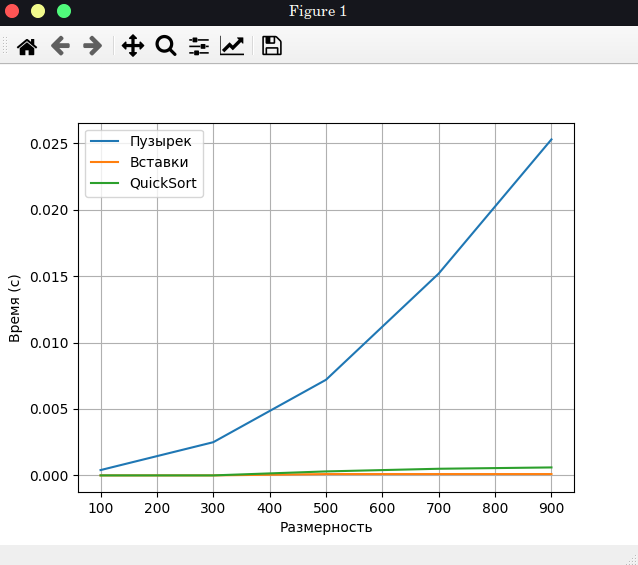
\includegraphics[width=0.8\textwidth]{img/best.png}
		\caption{Время работы алгоритмов на лучших данных.}
		\label{fg:ref3}}
\end{figure}

\begin{figure}[ht!]
	\centering{
		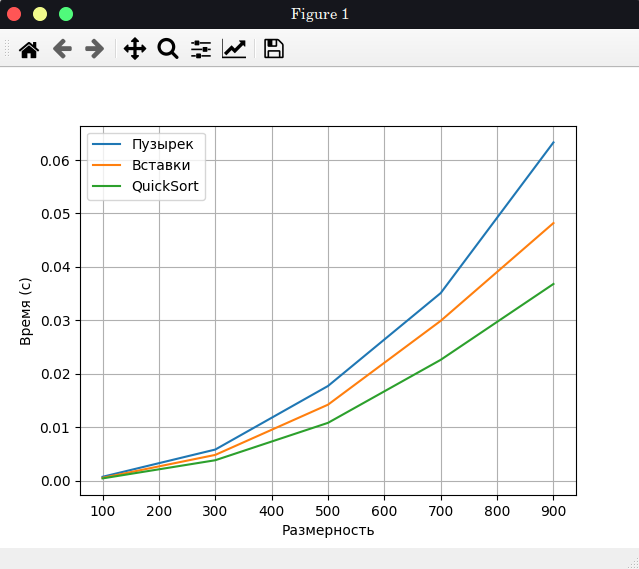
\includegraphics[width=0.8\textwidth]{img/worst.png}
		\caption{Время работы алгоритмов на худших данных.}
		\label{fg:ref4}}
\end{figure}

\begin{figure}[ht!]
	\centering{
		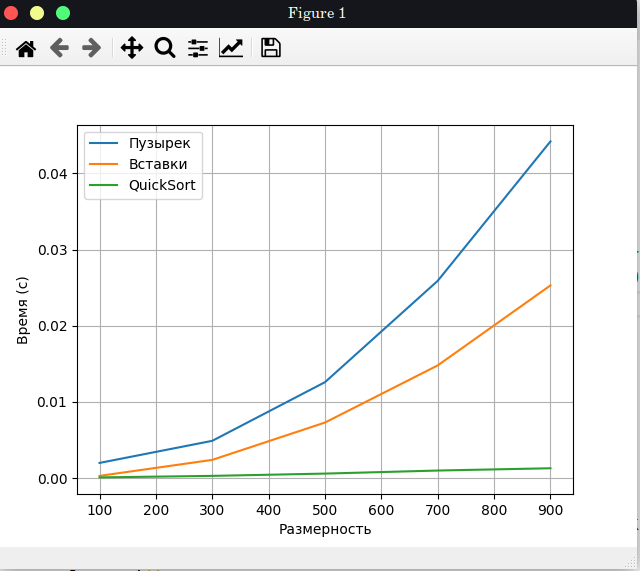
\includegraphics[width=0.8\textwidth]{img/random.png}
		\caption{Время работы алгоритмов на рандомных данных.}
		\label{fg:ref5}}
\end{figure}

\section{Сравнительный анализ алгоритмов}

Введем модель вычислений трудоемкости алгоритма.
Пусть трудоемкость 1 у следующих базовых операций: +, -, *, /, \%, =, ==, !=, <, <=, >, >=, [].
Трудоемкость цикла: fцикла = fиниц + fсравн + Nитер ∗ (fтела +
fинкрем + fсравн ).Трудоемкость условного перехода 1.

Алгоритм сортировки пузырьком обладает трудоемкостью \ref{eq:ref1}.

\begin{equation}
	N^2 * \left[ 
	\begin{array}{c}
		$4 л.с.$ \\
		$8.5 x.c$
	\end{array}
	\right.\\ 
	+ N * \left[ 
	\begin{array}{c}
		$3 л.с.$ \\
		$-1.5 x.c$
	\end{array}
	\label{eq:ref1}
	\right. - 4\\ 
\end{equation}

Трудоемкость квадратичная от размера массива. 

Сортировка вставками в лучшем случае, если уже отсортированный
массив: $О(N)$.
В худшем случае, если обратно отсортированный массив: $О(N^2)$.

Быстрая сортировка в лучшем случае: $О(N ∗ log(N))$.
В худшем случае: $О(N^2)$.

\section{Вывод}

Все алгоритмы в худшем случае обладают квадратичной сложностью.
А в лучшем случае меньше всего сложность у алгоритма сортировки
вставками.